\documentclass[12pt]{article}
\usepackage{amsthm,amsmath,amssymb,color}
\usepackage{tikz}
\usepackage{color}

\begin{document}

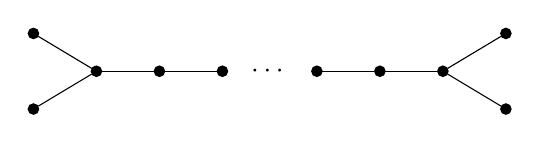
\begin{tikzpicture}
      [scale=.4,auto=left,every node/.style={scale=1}]
      \tikzset{Bullet/.style={circle,draw,fill=black,scale=0.4}}
      \node[Bullet] (uu) at (-5.5,0) {};
      \node[Bullet] (vv) at (5.5,0)  {};
      \node[Bullet] (u1) at (-7.5,1.2)  {};
      \node[Bullet] (u2) at (-7.5,-1.2)  {};
      \node[Bullet] (uu2) at (-3.5,0)  {};
      \node[Bullet] (vv2) at (3.5,0) {};
      \node[Bullet] (uu3) at (-1.5,0)  {};
      \node[Bullet] (vv3) at (1.5,0) {};
      \node[Bullet] (v1) at (7.5,1.2)  {};
      \node[Bullet] (vr) at (7.5,-1.2)  {};
      \node(dots) at (0,0){$\cdots$};

      \foreach \from/\to in {u1/uu, u2/uu, v1/vv,vr/vv,uu/uu2,uu2/uu3,vv/vv2,vv2/vv3}
        \draw[black] (\from) -- (\to);
    \end{tikzpicture}

\end{document}